\documentclass[a4paper,fleqn,12pt]{article}

\usepackage[utf8]{inputenc}
\usepackage[bulgarian]{babel}
\usepackage{amsmath}
\usepackage{amssymb}
\usepackage{booktabs}
\usepackage{fancyhdr}
\usepackage{amsthm}
\usepackage{graphicx}
\usepackage{pdfpages}
\usepackage{color}

%\pagestyle{fancy}
%\fancyhf{}
%\lhead{\rightmark}
%\rhead{\thepage}
%\cfoot{}
%\renewcommand{\headrulewidth}{0pt}

%\sloppy
%\definecolor{lightgray}{gray}{0.5}
%\setlength{\parindent}{0pt}



\begin{document}
\begin{titlepage}
	\setlength{\parindent}{0pt}
	\large
\centering
Технически университет -  София \par
Факултет по приложна математика и информатика \par
\vspace{2cm}

{\huge Курсова работа \par}

\vspace{2cm}

\vspace{1cm}
{\LARGE\scshape Числено моделиране с обикновенни диференциални уравнения \par}



\vfill

\begin{minipage}[t]{.5\linewidth}
	Студент: \\
	Кристиян Кръчмаров
\end{minipage}%
\begin{minipage}[t]{.5\linewidth}
	\raggedleft
	Преподавател:\\
	доц. д-р. Богдан Гилев
\end{minipage}

\vspace{2cm}
\raggedright

\end{titlepage}
\tableofcontents
\newpage

\section{Задачи}
\subsection{Задача 1}
Да се реши системата по Рунге - Кута: 
	\begin{gather}
		\begin{array}{|l@{}}
		\frac{dy_1}{dx} = y_2 \\
		\frac{dy_2}{dx} = f(x,y_1,y_2)
		\end{array} \qquad \qquad  \text{при} \qquad \qquad 
		\begin{array}{|l@{}}
		y_1(0) = 0\\
		y_2(0) = y_{20}
		\end{array}\\
		\text{където:} \nonumber \\
		f(x,y_1,y_2) = -axy_2 - x^2y_1 \quad a=0.05 \quad y_{20} = -\frac{1}{6} \nonumber
	\end{gather}
\subsection{Задача 2}
Да се сведе до система и да се реши по метода на матричната експонента уравнението при нулеви начални условия
	\begin{equation}
	y''+3y'=xe^{-2x}
	\end{equation}
\subsection{Задача 3}
Да се реши граничната задача по метода на крайните разлики
	\begin{equation}
	x'' + \frac{1}{t} x' + \left( \frac{16}{t^2}\right) x = \sin \left( \frac{1}{t^2}\right) \qquad t \in [1;4]; \, x(1) = -0.3 ; \, x(4) = 0.4
	\end{equation}
\subsection{Задача 4}
Да се реши граничната задача по метода на стрелбата
	\begin{equation}
	x'' + \frac{1}{t} x' + \left( \frac{16}{t^2}\right) x = \sin \left( \frac{1}{t^2}\right) \qquad t \in [1;4]; \, x(1) = -0.3 ; \, x(4) = 0.4
	\end{equation}
\newpage
\section{Решения}
\subsection{Задача 1}
Mетодът на Рунге-Кута от 4ти ред се използва за числено решение на система 
обикновенни диференциални уравнения от вида.
	\begin{gather*}
		\begin{array}{|l@{}}
		\frac{dy_1}{dx} = g(x,y_1,y_2) \\
		\frac{dy_2}{dx} = f(x,y_1,y_2)
		\end{array}
		\qquad \qquad  \text{при} \qquad \qquad 
		\begin{array}{|l@{}}
		y_1(x_0) = y_{10}\\
		y_2(x_0) = y_{20}
		\end{array} \\
		\text{където:}  \\
		y_1 = y_1(x) ; \, y_2 =y_2(x) 
	\end{gather*}
Методът се базира на апроксимация на следващата стойност на фунцкията, 
като използва няколко променливи за изчисляване на инкрементацията. 
При Метод на Рунге-Кута от 4ти ред се използват следните променливи
	\begin{gather*}
		k_{1,1} = h \cdot f(x_i,y_{1i}, y_{2i})\\
		k_{2,1} = h \cdot f \left(x_i + \frac{h}{2}, y_{1,i} + \frac{k_{1,1}}{2}, y_{2,i} + \frac{k_{1,2}}{2}\right)\\
		k_{3,1} = h \cdot f \left(x_i + \frac{h}{2}, y_{1,i} + \frac{k_{2,1}}{2}, y_{2,i} + \frac{k_{2,2}}{2}\right)\\
		k_{4,1} = h \cdot f \left(x_i + h, y_{1,i} + k_{3,1}, y_{2,i} + k_{3,2}\right)\\
		y_{1,i+1} = y_{1,i} + \frac{1}{6} \left( k_{1,1} +2k_{2,1} + 2k_{3,1} + k_{4,1}\right)h\\
		\\
		k_{1,2} = h \cdot g(x_i,y_{1i}, y_{2i})\\
		k_{2,2} = h \cdot g \left(x_i + \frac{h}{2}, y_{1,i} + \frac{k_{1,1}}{2}, y_{2,i} + \frac{k_{1,2}}{2}\right)\\
		k_{3,2} = h \cdot g \left(x_i + \frac{h}{2}, y_{1,i} + \frac{k_{2,1}}{2}, y_{2,i} + \frac{k_{2,2}}{2}\right)\\
		k_{4,2} = h \cdot g \left(x_i + h, y_{1,i} + k_{3,1}, y_{2,i} + k_{3,2} \right) \\
		y_{2,i+1} = y_{2,i} + \frac{1}{6} \left( k_{1,2} +2k_{2,2} + 2k_{3,2} + k_{4,2}\right)h\\
\end{gather*}
където $y_{1,i}$ и $y_{2,i}$ са предходни приближения, а $y_{1,i+1}$ и $y_{2,i+1}$ са текущи приближения. \\
	\newpage
	\begin{verbatim}
	function firstTask
	% Дефиниране на началните условия
	y0 = [0; -1/6];
	x0 = 0;
	% Дефиниране на стъпката и броя на стъпките
	h = 0.1;
	n = 100;
	% Използване на RK4 функцията
	[x, y] = RK4(@system, x0, y0, h, n);
	% Графика на резултатите
	plot(x,y(1,:),x,y(2,:));
	title('Решение на системата по Рунге-Кута');
	legend('y1', 'y2', 'Location', 'southwest', 'Orientation', 'vertical');
	xlabel('x');
	end
	
	function [x, y] = RK4(f, x0, y0, h, n)
	% f - функция, която връща дясната част на системата
	% x0 - начална точка за решението
	% y0 - началните условия
	% h - стъпка на метода
	% n - брой стъпки
	
	x = x0 + (0:n-1)*h;  % Изчисляваме x стойностите
	y = zeros(length(y0), n);  % Създаваме матрица за y
	y(:,1) = y0;  % Запазваме началните условия в първата колона на y
	for i = 1:n-1
	    k1 = f(x(i), y(:,i));
	    k2 = f(x(i)+0.5*h, y(:,i)+0.5*h*k1);
	    k3 = f(x(i)+0.5*h, y(:,i)+0.5*h*k2);
	    k4 = f(x(i)+h, y(:,i)+h*k3);
	    y(:,i+1) = y(:,i) + h*(k1+2*k2+2*k3+k4)/6;  % Изчисляваме y_i+1
	end
	end
	
	function dydx = system(x, y)
	a = 0.05;
	dydx = [y(2); -a*y(2) - x^2*y(1)];
	end
	\end{verbatim}

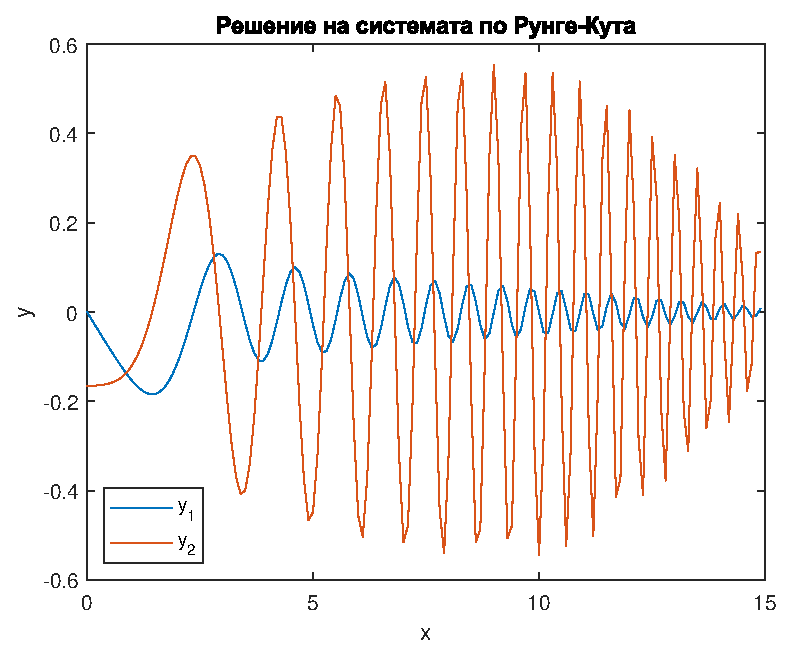
\includegraphics [width=4in]{firstTask_01.eps}

\newpage
\subsection{Задача 2}

\newpage
\subsection{Задача 3}

\newpage
\subsection{Задача 4}










































































\end{document}